\documentclass[a6paper, 10pt, twoside]{article}
%\usepackage[T1]{fontenc}
\usepackage[british]{babel}
\usepackage[utf8]{inputenc}
\usepackage{float, graphicx,amsmath,amsfonts,cite,enumerate}
\usepackage[final]{pdfpages}
\usepackage{wrapfig}
\usepackage[margin=0.3in]{geometry}
\usepackage{sidspaltHack}
\usepackage{digital}

\setlength{\oddsidemargin}{-0.37in}
\setlength{\evensidemargin}{-0.47in}
\setlength{\textwidth}{215pt}

\pagestyle{empty}

\begin{document}
\nysida{8}{}
\noindent
\chaptertitle{$\Theta\theta$}{Blöta visor}
\newline
\large\textit{\indent Vem jämrar och stönar? Vem grälar och bråkar? Vem skaffar sig onödiga sår och får simmiga ögon? \\
\indent Den som blir sittande vid glaset, den som kommer för att smaka det kryddade vinet. \\
\indent Se inte på vinet som skimrar rött, som glittrar i bägaren
och rinner ner så lätt.\\
\indent Till slut biter det som en orm,
hugger som en giftorm. \\
\indent Då ser du underliga syner och får \\befängda idéer:\\
\indent än ligger du mitt ute i havet, än högt uppe i mastkorgen.\\
\indent "De slog mig men det gjorde inte ont,
jag fick stryk men märkte det inte.
När skall jag vakna?
Jag vill ha mer!"}
\auth{Ordspråksboken 23:29-35}


\small % TODO: Scope the above \large tags, so that we don't need renewal of \small here.
\nysida{8}{1}
\begin{center}
\songtitle{$\theta1$}{Störthärligt full} 
\mel{Fat mamie Brown}
\end{center}
\begin{lyrics}
Nu har alla lämnat festen och jag \\
sitter ensam kvar,\\
ibland groggar, pilsnerflaskor\\
i en sönderslagen bar.\\
Första pilsnerflaskan tog jag vid\\
min frukost klockan fem,\\
och nu sitter jag och väntar på att\\
få bli buren hem.
\vspace{5pt}\\
\textbf{För jag är störthärligt full\\
och jag ramlar mest omkull,\\
och jag ser skära elefanter,\\
som har jättekonstig ull.\\
Ja, jag är är störthärligt full\\
och jag ramlar mest omkull\\
och det är präktigt härligt\\
att supa och va' full.}
\vspace{5pt}\\
Ifrån festen minns jag inget - jo\\
mitt öga blev visst blått,\\
och det måste jag ha fått när\\
någon kasta' en karott.\\
Full med vispgrädde och\\
fimpar och en okammad peruk,\\
eller också när jag stod i moraklockan\\
och var sjuk.
\vspace{5pt}\\
\textbf{För jag är störthärligt full...}
\newpage
\noindent
Och i morgon när jag vaknar -\\
med en bergsborr i min kropp,\\
sandpapper på tungan och\\
jag vill ej stiga opp.\\
Mina armar de känns tunga\\
och min näsa den är sne',\\
så jag raglar ut till köket\\
för en återställare!
\vspace{5pt}\\
\textbf{För jag är störthärligt full...}
\end{lyrics}
\auth{Hittad på Handels 1981}
\sidindex{8}{2}
\begin{center}
\songtitle{$\theta2$}{Jag var full en gång} 
\mel{Flottarkärlek}
\end{center}
\begin{lyrics}
Jag var full en gång för länge se'n. \\
På knäna kröp jag hem, \\
varje dike var för mig ett vilohem. \\
I varje hörn och varje vrå \\
där hade jag en liten vän, \\
ifrån renat upp till nittiosex procent. 
\vspace{5pt}\\
Jag var full en gång för länge se'n. \\
På knäna kröp jag hem \\
och i sällskap hade jag en elefant. \\
Elefanten spruta' vatten \\
och jag trodde det var öl. \\
Sedan dess har alla kallat mig för knöl -- fylleknöl!
\digitalonly{\newline\newline\newline Andra versen kan upprepas med "öl-fylleknöl" utbytt mot "vin-fyllesvin", och sedan "sprit-fylleskit"}
\end{lyrics}
\vspace{5pt}\\ % TODO: Digitalize
\textit{Andra versen kan upprepas med "öl-fylleknöl" utbytt mot \textbf{vin-fyllesvin}, \textbf{sprit-fylleskit} och\\ \textbf{pisang-fylleslang}}

\nysida{8}{3}
\begin{center}
\songtitle{$\theta3$}{Bär ner mig till sjön} 
\mel{Bei mir bist du schön}
\end{center}
\begin{lyrics}
$\|$: Bär ner mig till sjön, \\
bär ner mig till sjön, \\
jag känner att jag måste i! :$\|$ \\
Och när du badat mig, \\
så skall du torka mig. \\
Och när du torkat mig, \\
så vill jag i igen! 
\vspace{5pt}\\
$\|$: Bär upp mig i en tall,\\
bär upp mig i en tall,\\
jag känner att jag måste upp! :$\|$ \\
Och när jag kommit upp,\\
så vill jag ner igen. \\
och när jag kommit ner,\\
så vill jag upp igen! 
\vspace{5pt}\\
$\|$: Häll i mig min grogg,\\
häll i mig min grogg,\\
jag känner att jag tål det väl. :$\|$\\
Och när jag fått min grogg, \\
så fyll då på igen. \\
Och när du fyllt mitt glas, \\
så häll då i igen! 
\vspace{5pt}\\
$\|$: Bär ut mig i snön, \\
bär ut mig i snön, \\
jag känner att jag måste spy. :$\|$ \\
Och när jag kastat upp, \\
så får du torka opp. \\
Och när du torkat upp, \\
så kan jag spy igen.!

\newpage
\noindent
$\|$: Var var jag igår? \\
Var var jag igår? \\
Jag undrar, var var jag igår? :$\|$\\
Mitt huvud känns så tungt, \\
jag kan ej andas lugnt. \\
Hur har jag kommit hem? \\
Och vem har stoppat mig i säng? 
\end{lyrics}
\vspace{10pt}
\sidindex{8}{4}
\begin{center}
\songtitle{$\theta4$}{Minne} 
\mel{Memories (Cats)}
\end{center}
\begin{lyrics}
Minne, jag har tappat mitt minne! \\
Är jag svensk eller finne?\\
Kommer inte ihåg...
\vspace{5pt}\\
Inne, är jag ut eller inne?\\
Jag har luckor i minnet,\\
sådär små alko-hål.\\
Men besinn' er,\\
en tätar med det brännvin en får\\
fastän minnet och helan går. 
\end{lyrics}
\vspace{10pt}
\begin{center}
\songtitle{$\theta5$}{Antisnapsvisa} 
\mel{Sjösala vals}
\end{center}
\begin{lyrics}
Huvudet vi lyfter med ett stön ur vår säng.\\
Diskmaskin i buken, kanoner i huvudet.\\
Tungan som en plyschsoffa och yrseln i sväng.\\
I ångesten vi svettas, kom sjung din refräng.
\vspace{5pt}\\
Varför finns det aldrig någon nykter QuArneVal?\\
O, låt oss somna om så vi slipper våra kval.\\
Men se, så många supar vi redan kastat upp i sängen:\\
Renat och Skåne, Svartvinbär och fager Bäsk! 
\end{lyrics}

\nysida{8}{6}
\begin{center}
\songtitle{$\theta6$}{Dom som är nyktra} 
\mel{Du är den ende}
\end{center}
\begin{lyrics}
Dom som är nyktra,\\
de har inge' roligt.\\
Dom har bara ansvar\\
och inte nå't tjolit-\\
an-lej-faderulla.\\
Men vi som är fulla\\
vi har bara kul nästan jämt.
\vspace{5pt}\\
Det sägs att en mänska\\
kan va' utan brännvin.\\
Det stämmer kanhända,\\
men se blott på den min\\
som pryder en absolutist.\\
Den är jävligt trist,\\
därför så sjunger vi så:
\vspace{5pt}\\
Dom som är nyktra ...
\vspace{5pt}\\
Dom som är rika\\
har mynt så det räcker.\\
Ur de som är harmynt-\\
a brännvinet läcker.\\
När de tar en hela\\
ses gommen sig dela.\\
Så därför är jag hellre rik än harmynt! 
\begin{center}\textit{Vers att sjunga i dur\digitalonly{:}}\end{center}\physicalonly{
}Det gör det samma var vi må va' gäster.\\
Ja, till och med lanthushållningssällskapsfester\\
kan uthärdas med eau-de-vie\\
som får månda'n att bli blott en vag utopi.
\end{lyrics}

\nysida{8}{7}
\begin{center}
\songtitle{$\theta7$}{Treo-comp} 
\mel{Längtan till landet}
\end{center}
\begin{lyrics}
Morgonstund med smak av döda bävrar\\
frukostmorgonen är över oss.\\
Hur vi alla stretar, hur vi vägrar\\
så går solen lik förbannat opp.
\vspace{5pt}\\
Snart är dagen här med hemska plågor\\
huvudvärk, yrsel, elände men,\\
det finns faktiskt ett glas som dej kan rädda.\\
Treo-comp vår frälsare och vän. 
\end{lyrics}
\vspace{40pt}
\begin{center}
\songtitle{$\theta8$}{Vit vecka} 
\mel{White christmas}
\end{center}
\begin{lyrics}
Jag drömmer om en vit vecka.\\
Sju dagar utan alkohol.\\
Tänk att bara skåla\\
i juice och cola\\
och sedan minnas allt en gjort.
\vspace{5pt}\\
Jag drömmer om en vit vecka.\\
Det finns en gräns för vad jag tål.\\
Jag vill inte ha mera sprit,\\
så låt nästa vecka vara vit.
\end{lyrics}
\auth{Sångarstriden 1992} 

\nysida{8}{9}
\begin{center}
\songtitle{$\theta9$}{Vi dricka, vi dricka} 
\mel{Tre Pepparkaksgubbar}
\end{center}
\begin{lyrics}
Vi dricka, vi dricka\\
upp allt som dukas fram.\\
Först ölen och vinet\\
sen snapsar vi som f-n.\\
Väl runda och goda\\
vi lämnar vår salong.\\
Men ramlar ner och somnar sött\\
i rännstenens schäslong.
\end{lyrics}
\auth{David Danowsky (F)}
\vspace{40pt}
\begin{center}
\songtitle{$\theta10$}{When I get drunker}
\mel{When I'm 64} 
\end{center}
\begin{lyrics}
When I get drunker, loosing my mind\\
many beers from now.\\
Will I still be having me a jolly good time,\\
whisky, gin and a bottle of wine.\\
So, fill up the glasses, drunk as a skunk,\\
don't say you want no more,\\
'cause we are the singers\\
and we are the swingers,\\
join us and you won't get bored.
\end{lyrics}

\nysida{8}{11}
\begin{center}
\songtitle{$\theta11$a}{Vi ska supa}
\mel{Askungen}
\end{center}
\begin{lyrics}
Vi ska supa, vi ska festa,\\
vi ska göra vårat bästa,\\
vi ska låta marken gunga,\\
vi äro ännu unga.\\
Vi dansar uppå borden\\
vi festar in Norden\\
och vi ska bara supa, sjunga, \\
spexa, älska, vara unga.\\
Imorgon äro alla huven tunga.
\end{lyrics}
\begin{center}
\vspace{20pt}
\songtitle{$\theta11$b}{Härjarens bordsvisa}
\mel{Askungen}
\end{center}
\begin{lyrics}
Vi ska röja, vi ska härja\\
vi ska supa, slåss och svärja.\\
Oss förnöja sisådärja\\
med blod vi knappt oss värja\\
kan från ett "Bloody-Mary"-a.\\
Nu änteligen lär ja'\\
dra någon riktig nytta av\\
min gamla brännvinsautoklav\\
och om det så ska bli min grav\\
min sprit förtär ja'.
\vspace{5pt}
La la la...
\end{lyrics}
\auth{Bordsvisa Sångarstriden 1985, Lund}

\nysida{8}{12}
\begin{center}
\songtitle{$\theta12$}{Selen lever}
\mel{He's got the whole world in his hand}
\end{center}
\begin{lyrics}
\textbf{$\|$: Selen lever, i vår hånd :$\|$ x4}
\vspace{5pt}\\
Vi stikker hakkapikken i den, i vår sel...
\vspace{5pt}\\
\textbf{Men! Selen lever...}
\vspace{5pt}\\
Vi river skinnet av den, av vår sel...
\vspace{5pt}\\
\textbf{Men! Selen lever...}
\vspace{5pt}\\
Vi river loffene av den, av vår sel...
\vspace{5pt}\\
\textbf{Men! Selen lever...}
\vspace{5pt}\\
Vi river tarmene ut av den, av vår sel...
\vspace{5pt}\\
\textbf{Men! Selen lever...}
\vspace{5pt}\\
Vi stikker øynere ut av den, av vår sel...
\vspace{5pt}\\
\textbf{Men! Selen lever...}
\vspace{5pt}\\
Vi kjører speedbåt over den, på vår sel...
\vspace{5pt}\\
\textbf{Men! Selen lever...}
\vspace{5pt}\\
Carl Gustaf gråter, för vår sel... 
\end{lyrics}
\begin{figure}[!h]
\hfill 
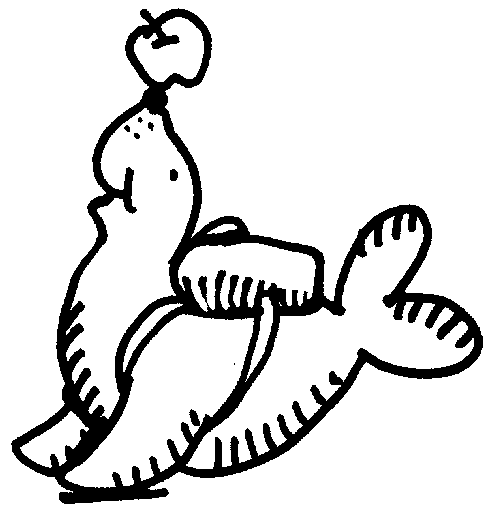
\includegraphics[width=0.5\textwidth]{seal.png}
\end{figure}
\end{document}